\section{Finite Difference Method}

\begin{bigidea}
Most differential equations are impossible to solve exactly and so we use numerical methods such as the finite difference method to approximate solutions. The finite difference method applied to a linear differential equations yields a linear system of equations $A \bs{y} = \bs{b}$.
\end{bigidea}

\begin{definition}
An \href{https://en.wikipedia.org/wiki/Differential_equation}{\bf ordinary differential equation} is an equation involving an unknown function $y(t)$ and its derivatives. The {\bf order} of a differential equation is the highest order derivative appearing in the equation. There are many kinds of differential equations. In this section, we consider only {\bf second order linear ordinary differential equations}
$$
y'' + p(t)y' + q(t)y = r(t)
$$
{\bf Boundary conditions} are equations imposed on the solution at the boundary points $t_0$ and $t_f$. For example, specify values of the solution $y(t)$ at the endpoints
$$
y(t_0) = \alpha \hspace{5mm} y(t_f) = \beta
$$
or specify a value of the solution $y(t)$ at one endpoint and a value of the derivative $y'(t)$ at the other endpoint
$$
y'(t_0) = \alpha \hspace{5mm} y(t_f) = \beta
$$
\end{definition}

\begin{definition}
The \href{https://en.wikipedia.org/wiki/Taylor_series}{\bf Taylor series} of a smooth function $f(x)$ centered at $x=a$ is
$$
f(x) = \sum_{n=0}^{\infty} \frac{f^{(n)}(a)}{n!} (x-a)^n = f(a) + f'(a)(x-a) + \frac{f''(a)}{2}(x-a)^2 + \frac{f'''(a)}{6}(x-a)^3 + \cdots
$$
\end{definition}

\begin{definition}
\href{https://en.wikipedia.org/wiki/Finite_difference}{\bf Finite difference formulas} are derived from Taylor series. Let $y(t)$ be a smooth function and consider the Taylor series
\begin{align*}
y(t+h) &= y(t) + y'(t)h + \frac{y''(t)}{2}h^2 + \cdots \\
y(t-h) &= y(t) - y'(t)h + \frac{y''(t)}{2}h^2 + \cdots
\end{align*}
Truncate and rearrange the first series for the {\bf forward difference formula}
$$
y'(t) \approx \frac{y(t+h) - y(t)}{h}
$$
Truncate and rearrange the second series for the {\bf backward difference formula}
$$
y'(t) \approx \frac{y(t) - y(t - h)}{h}
$$
Subtract $y(t+h) - y(t-h)$ and truncate to get the (first order) {\bf central difference formula}
$$
y'(t) \approx \frac{y(t+h) - y(t-h)}{2h}
$$
Add $y(t+h) + y(t-h)$ and truncate to get the (second order) {\bf central difference formula}
$$
y''(t) \approx \frac{y(t+h) -2y(t) + y(t-h)}{h^2}
$$
\end{definition}

\begin{definition}
The {\bf finite difference method} applied to a second order linear ordinary differential equation with boundary conditions 
$$
y'' + p(t)y' + q(t)y = r(t) \ \ , \ \ t \in [t_0,t_f]
$$
\begin{enumerate}
\item Discretize the domain: choose $N$, let $\ds h = \frac{t_f - t_0}{N+1}$ and define $t_k = t_0 + kh$.
\item Let $y_k \approx y(t_k)$ denote the approximation of the solution at $t_k$.
\item Substitute finite difference formulas into the equation to define an equation at each $t_k$.
\item Rearrange the system of equations into a linear system $A \bs{y} = \bs{b}$ and solve for
$$
\bs{y} = \begin{bmatrix} y_1 & y_2 & \cdots & y_N \end{bmatrix}^T
$$
\end{enumerate}
\end{definition}

\begin{example}
Consider a second order linear ordinary differential equation with boundary conditions of the form
$$
y'' = r(t) \ \ , \ \ y(t_0) = \alpha \ , \ \ y(t_f) = \beta
$$
Choose $N$ and let  $\ds h = \frac{t_f - t_0}{N+1}$ and define $t_k = t_0 + kh$. Let $y_k$ denote an approximation of $y(t_k)$. Note that the boundary conditions give us $y_0 = \alpha$ and $y_{N+1} = \beta$ and let
$$
\bs{y} = \begin{bmatrix} y_1 & y_2 & \cdots & y_N \end{bmatrix}^T
$$
Let $r_k = r(t_k)$ and substitute the central difference formula at $t_k$ into the differential equation
$$
\frac{y_{k+1} -2y_k + y_{k-1}}{h^2} = r_k
$$
Therefore we have $N$ equations and $N$ unknowns $y_k$ for $k=1,\dots,N$. Use the boundary conditions $y_0 = \alpha$ and $y_{N+1} = \beta$ and rearrange the equations
$$
\begin{array}{rrrrrrcrrrrcc}
- 2y_1 & + & y_2 & & & & & & & & & = & h^2 r_1 - \alpha \\
y_1 & - & 2y_2 & + & y_3 & & & & & & & = & h^2 r_2 \\
& & y_2 & - & 2y_3 & + & y_4 & & & & & = & h^2 r_3 \\
& & & & & & \ddots & & & & & \vdots & \\
& & & & & & y_{N-2} & - & 2y_{N-1} & + & y_N & = & h^2 r_{N-1} \\
& & & & & & & & y_{N-1} & - & 2y_N & = & h^2 r_N - \beta
\end{array}
$$
Rewrite in matrix form $A \bs{y} = \bs{b}$ where
$$
A =
\left[ \begin{array}{rrcrr}
-2 & 1 & & & \\
1 & -2 & 1 & & \\
& & \ddots & & \\
& & 1 & -2 & 1 \\
& & & 1 & -2
\end{array} \right]
\hspace{10mm}
\bs{b} = 
\begin{bmatrix}
h^2 r_1 - \alpha \\ h^2 r_2 \\ \vdots \\ h^2 r_{N-1} \\ h^2 r_N - \beta
\end{bmatrix}
$$
\end{example}

\begin{example}
Setup a linear system $A \bs{y} = \bs{b}$ for the equation with boundary conditions
$$
y'' = -2 \ \ , \ \ y(0) = 0 \ , \ \ y(1) = 0
$$
using step size $h=0.2$. \\

The step size $h$ corresponds to $N=4$ in our formulation, and $r(t) = -2$, $\alpha = \beta = 0$ therefore
$$
\left[ \begin{array}{rrrr}
-2 & 1 & & \\
1 & -2 & 1 & \\
& 1 & -2 & 1 \\
& & 1 & -2
\end{array} \right]
\begin{bmatrix} y_1 \\ y_2 \\ y_3 \\ y_4 \end{bmatrix}
=
\begin{bmatrix} -0.08 \\ -0.08 \\ -0.08 \\ -0.08 \end{bmatrix}
$$
Solve the system to find
$$
\begin{bmatrix} y_1 \\ y_2 \\ y_3 \\ y_4 \end{bmatrix}
=
\begin{bmatrix} 0.16 \\ 0.24 \\ 0.24 \\ 0.16 \end{bmatrix}
$$
The equation is very simple and we can solve exactly by integrating twice
$$
y(t) = -t^2 + C_1t +C_2
$$
The boundary conditions imply $C_1 = 1$ and $C_2 = 0$ and therefore the exact solution is
$$
y(t) = t - t^2
$$
Notice that our finite difference approximation found the exact values $y(0.2) = 0.16$, $y(0.4) = 0.24$, $y(0.6) = 0.24$, $y(0.8) = 0.16$. This is because our equation is very simple and the solution is a polynomial of degree 2. The finite difference method does not compute exact values in general.
\begin{center}
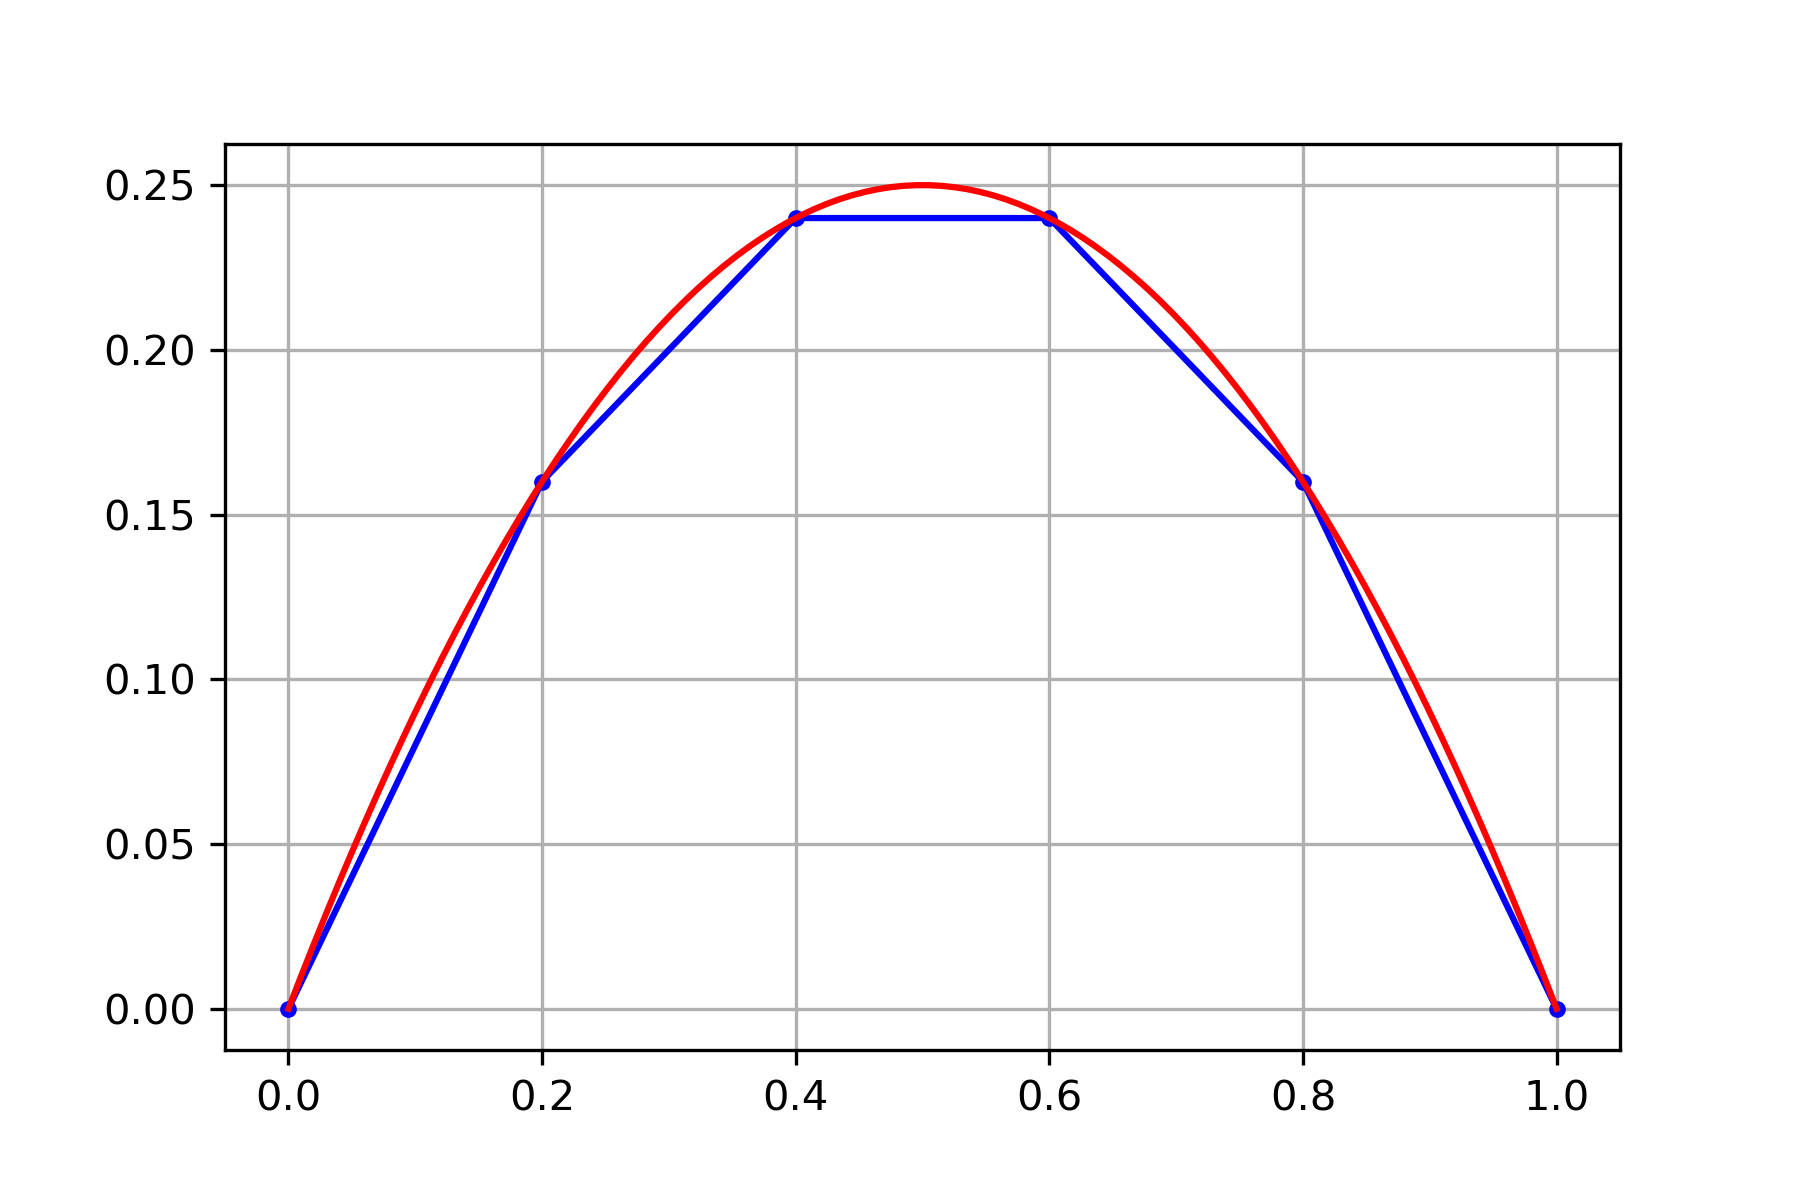
\includegraphics[width=4in]{01_08_img01.png}
\end{center}
\end{example}

\begin{example}
Setup a linear system $A \bs{y} = \bs{b}$ for the equation with boundary conditions
$$
y'' = \cos(t) \ \ , \ \ y(0) = 0 \ , \ \ y(2\pi) = 1
$$
using 7 equally spaced points from $t_0 = 0$ to $t_f = 2\pi$. \\

The value $N=5$ corresponds to 7 equally spaced points in our formulation with step size
$$
h = \frac{t_f - t_0}{N + 1} = \frac{2\pi - 0}{5 + 1} = \frac{\pi}{3}
$$
We have $r(t) = \cos(t)$ and $\alpha = 0$ and $\beta = 1$. Note that $r_k = \cos(k\pi/3)$ therefore
$$
\left[ \begin{array}{rrrrr}
-2 & 1 & & & \\
1 & -2 & 1 & & \\
& 1 & -2 & 1 & \\
& & 1 & -2 & 1 \\
& & & 1 & -2
\end{array} \right]
\begin{bmatrix} y_1 \\ y_2 \\ y_3 \\ y_4 \\ y_5 \end{bmatrix}
=
\begin{bmatrix} \pi^2/18 \\ -\pi^2/18 \\ -1 \\ -\pi^2/18 \\ \pi^2/18 - 1 \end{bmatrix}
$$
Use {\tt scipy.linalg.solve} to compute the solution. The equation is elementary and we can solve exactly by integrating twice
$$
y(t) = 1 - \cos(t) + \frac{t}{2 \pi}
$$
Plot the exact solution together with our approximation
\begin{center}
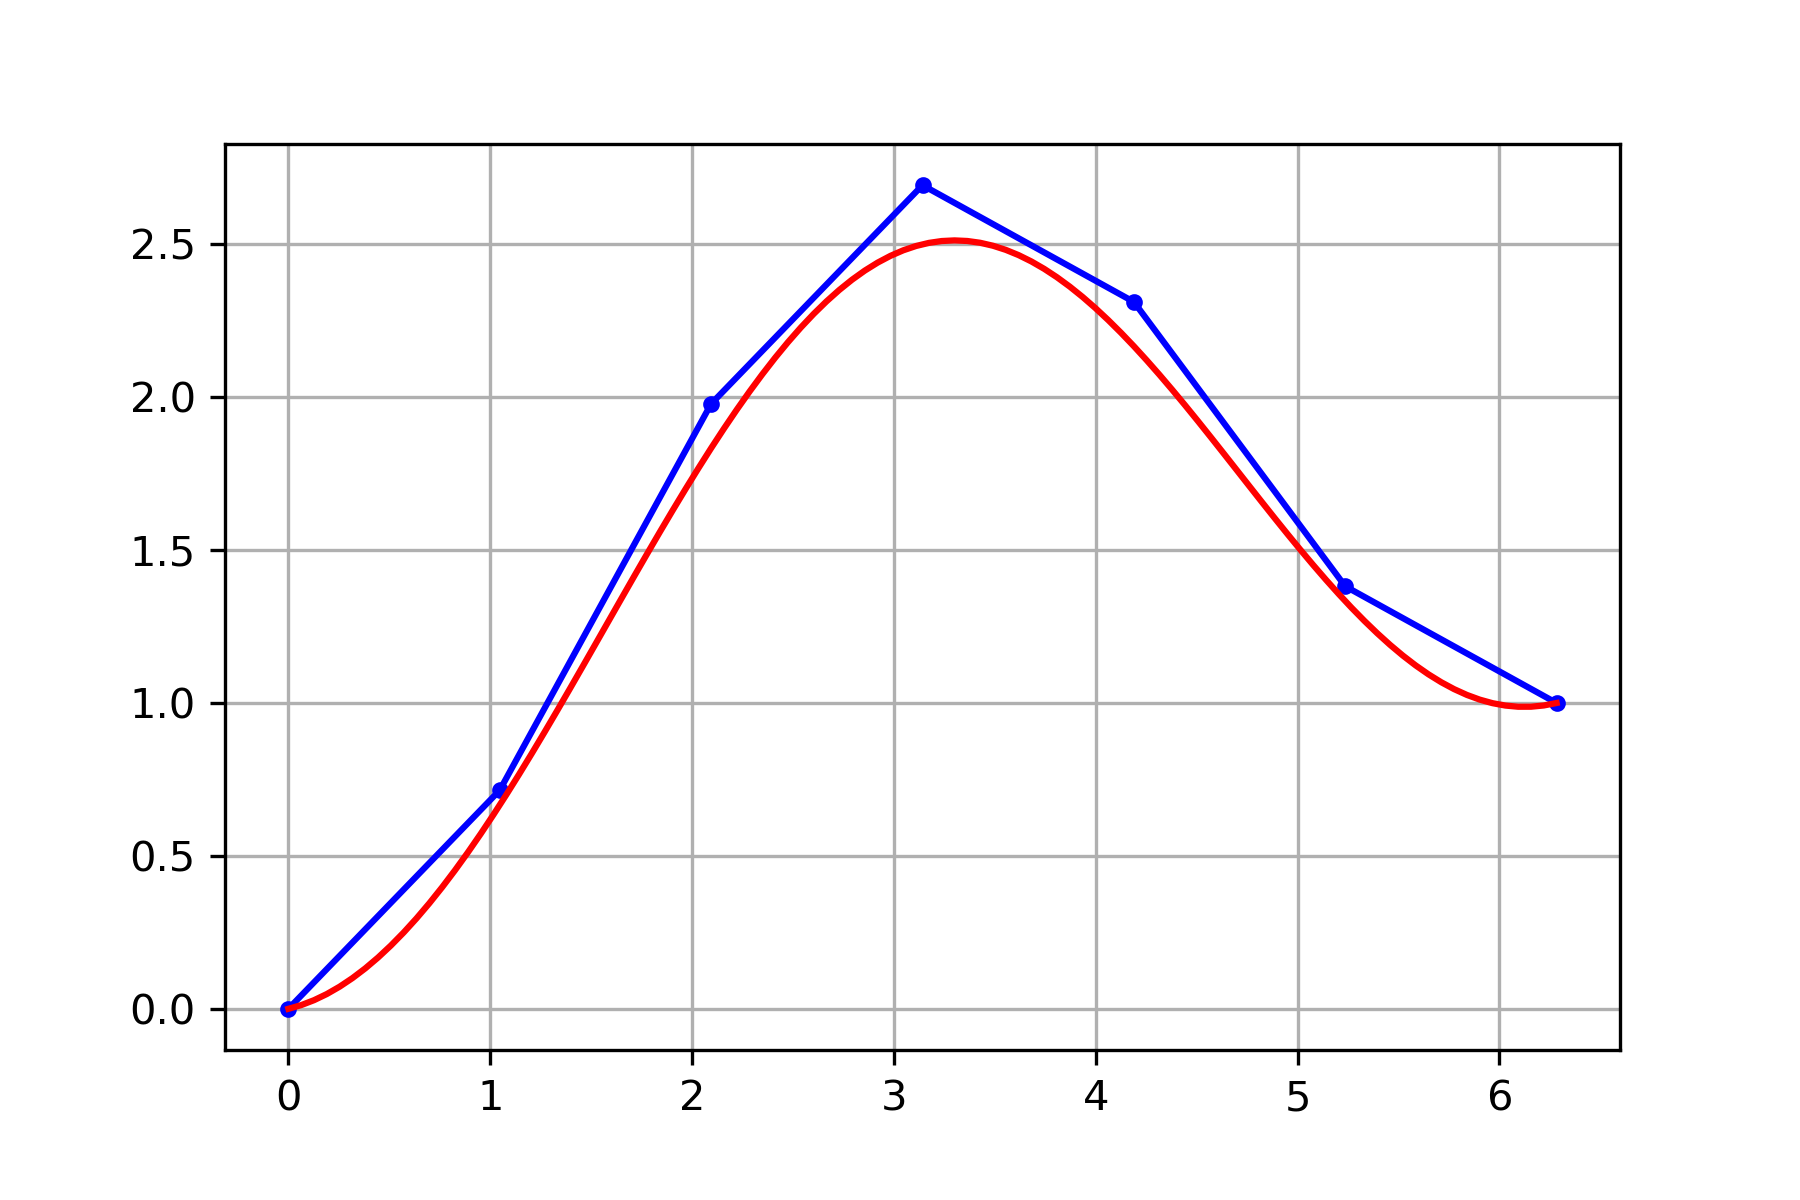
\includegraphics[width=4in]{01_08_img02.png}
\end{center}
\end{example}

\begin{note}
Increasing the number of points in the discretization (equivalently, decreasing the step size $h$) decreases the error but increases the number of computations. This is a general principle in numerical computing: {\it higher accuracy requires more computations}. For example, consider the same equation as the previous example
$$
y'' = \cos(t) \ \ , \ \ y(0) = 0 \ , \ \ y(2\pi) = 1
$$
but now use 21 equally spaced points from $t_0 = 0$ to $t_f = 2\pi$. Then $N=19$ and
$$
h = \frac{t_f - t_0}{N + 1} = \frac{2\pi - 0}{19 + 1} = \frac{\pi}{10}
$$
and the finite difference method produces a much better solution
\begin{center}
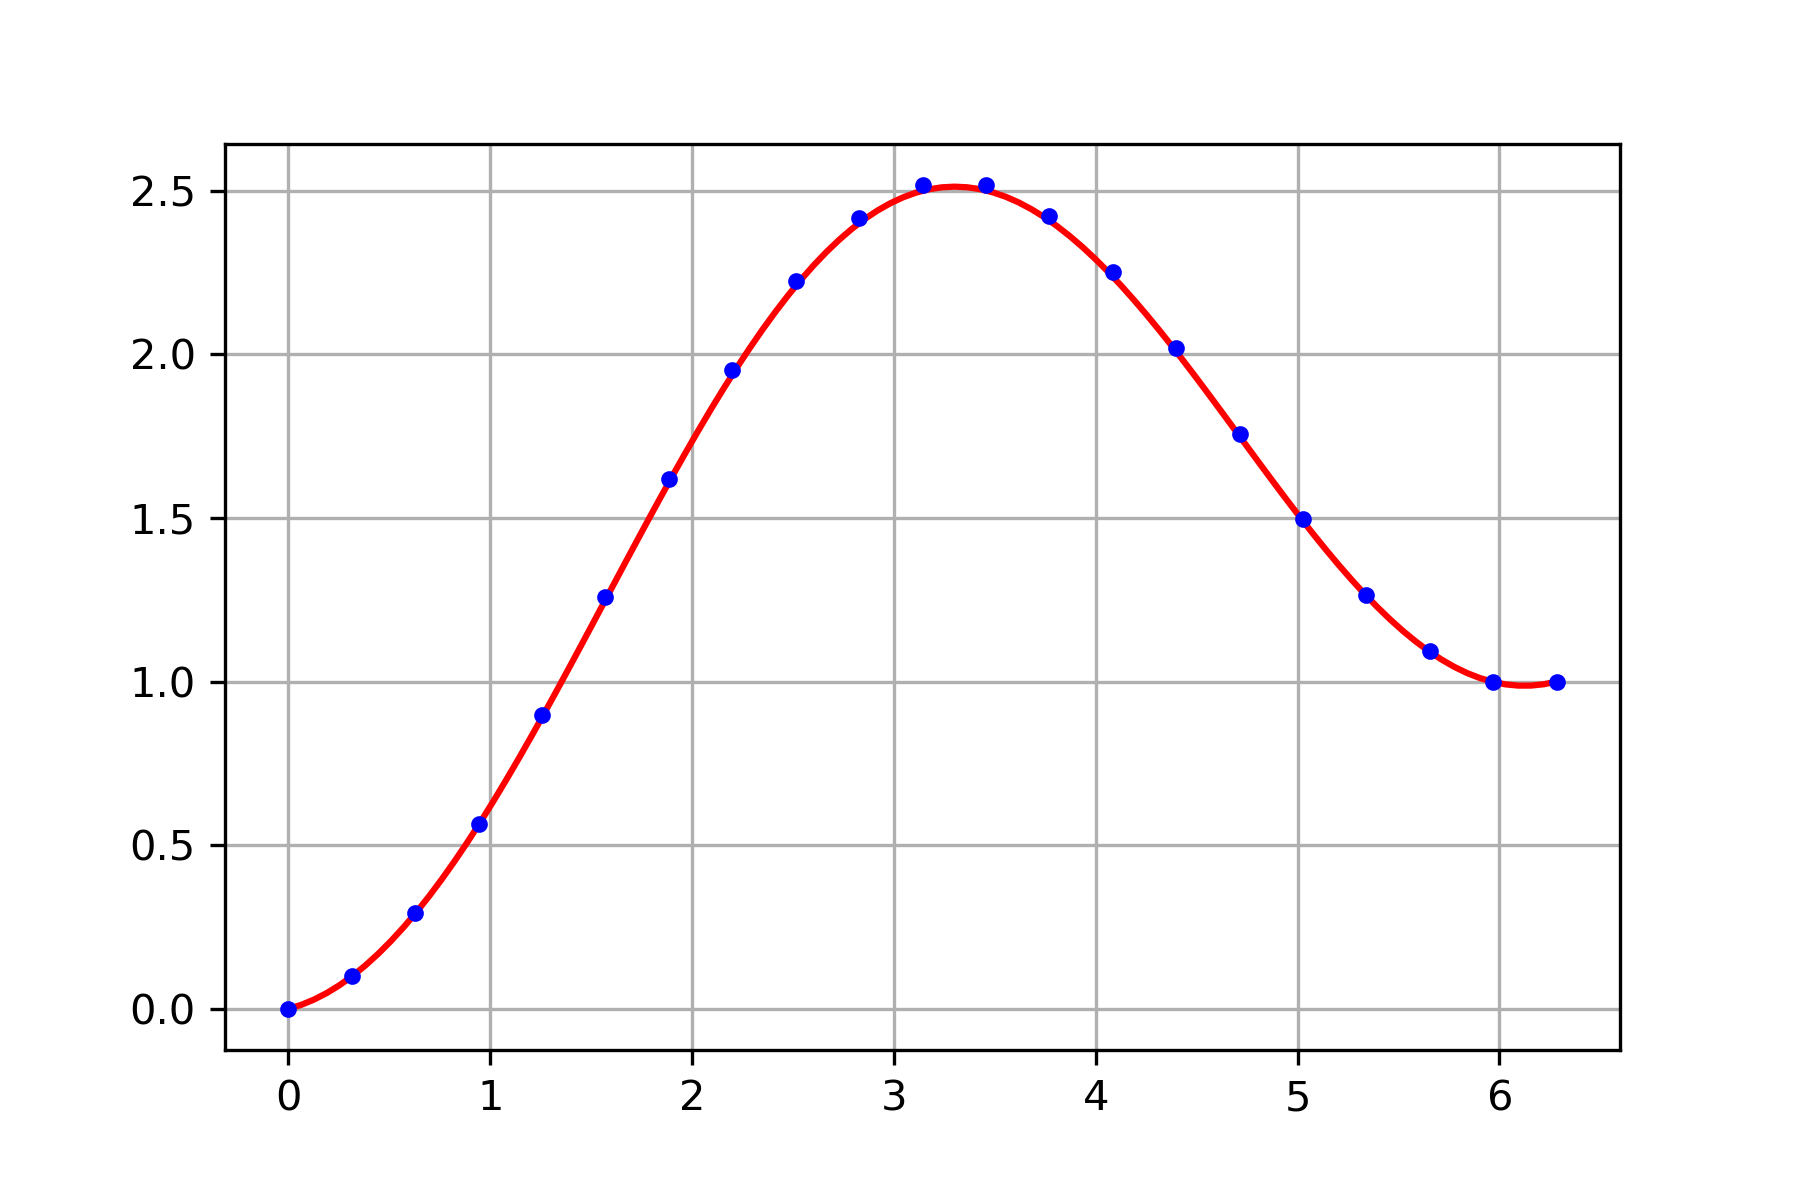
\includegraphics[width=4in]{01_08_img03.png}
\end{center}
\end{note}

\begin{example}
Consider the general form of a second order linear ordinary differential equation with boundary conditions
$$
y'' + p(t)y' + q(t)y = r(t) \ \ , \ \ y(t_0) = \alpha \ , \ \ y(t_f) = \beta
$$
Choose $N$ and let  $\ds h = \frac{t_f - t_0}{N+1}$ and define $t_k = t_0 + kh$. Let $y_k$ denote an approximation of $y(t_k)$. Note that the boundary conditions give us $y_0 = \alpha$ and $y_{N+1} = \beta$ and let
$$
\bs{y} = \begin{bmatrix} y_1 & y_2 & \cdots & y_N \end{bmatrix}^T
$$
Let $p_k = p(t_k)$, $q_k = q(t_k)$ and $r_k = r(t_k)$, and substitute the central difference formulas for both $y''$ and $y'$ at $t_k$ into the differential equation
$$
\frac{y_{k+1} -2y_k + y_{k-1}}{h^2} + p_k \frac{y_{k+1} - y_{k-1}}{2h} + q_k y_k = r_k
$$
Rearrange the equation
\begin{align*}
y_{k+1} -2y_k + y_{k-1} + \frac{h p_k}{2} \left( y_{k+1} - y_{k-1} \right) + h^2q_k y_k &= h^2 r_k \\
\left( 1 - \frac{h p_k}{2} \right) y_{k-1} + (h^2q_k - 2)y_k + \left(1 + \frac{h p_k}{2} \right)y_{k+1} &= h^2 r_k
\end{align*}
Introduce the notation
$$
a_k = 1 - \frac{h p_k}{2}
\hspace{10mm}
b_k = h^2q_k - 2
\hspace{10mm}
c_k = 1 + \frac{h p_k}{2}
$$
Use the boundary conditions $y_0 = \alpha$ and $y_{N+1} = \beta$ and rearrange the equations
$$
\begin{array}{rrrrcrrrrcc}
b_1 y_1 & + & c_1 y_2 & & & & & & & = & h^2 r_1 - \left( 1 - h p_1/2 \right) \alpha \\
a_2 y_1 & + & b_2 y_2 & + & c_2 y_3 & & & & & = & h^2 r_2 \\
& & & & \ddots & & & & & \vdots & \\
& & & & a_{N-1}y_{N-2} & + & b_{N-1}y_{N-1} & + & c_{N-1}y_N & = & h^2 r_{N-1} \\
& & & & & & a_Ny_{N-1} & + & b_Ny_N & = & h^2 r_N - \left( 1 + h p_N/2 \right) \beta
\end{array}
$$
Rewrite in matrix form $A \bs{y} = \bs{b}$ where
$$
A =
\left[ \begin{array}{rrcrr}
b_1 & c_1 & & & \\
a_2 & b_2 & c_2 & & \\
& & \ddots & & \\
& & a_{N-1} & b_{N-1} & c_{N-1} \\
& & & a_N & b_N
\end{array} \right]
\hspace{10mm}
\bs{b} = 
\begin{bmatrix}
h^2 r_1 - \left( 1 - h p_1/2 \right) \alpha \\ h^2 r_2 \\ \vdots \\ h^2 r_{N-1} \\ h^2 r_N - \left( 1 + h p_N/2 \right) \beta
\end{bmatrix}
$$
\end{example}

\begin{example}
Consider the differential equation with boundary conditions
$$
y'' + t^2y' + y = \cos(t) \ \ , \ \ y(0) = 0 \ , \ \ y(3) = 0
$$
Solving the linear system derived above with $N=19$ produces the result
\begin{center}
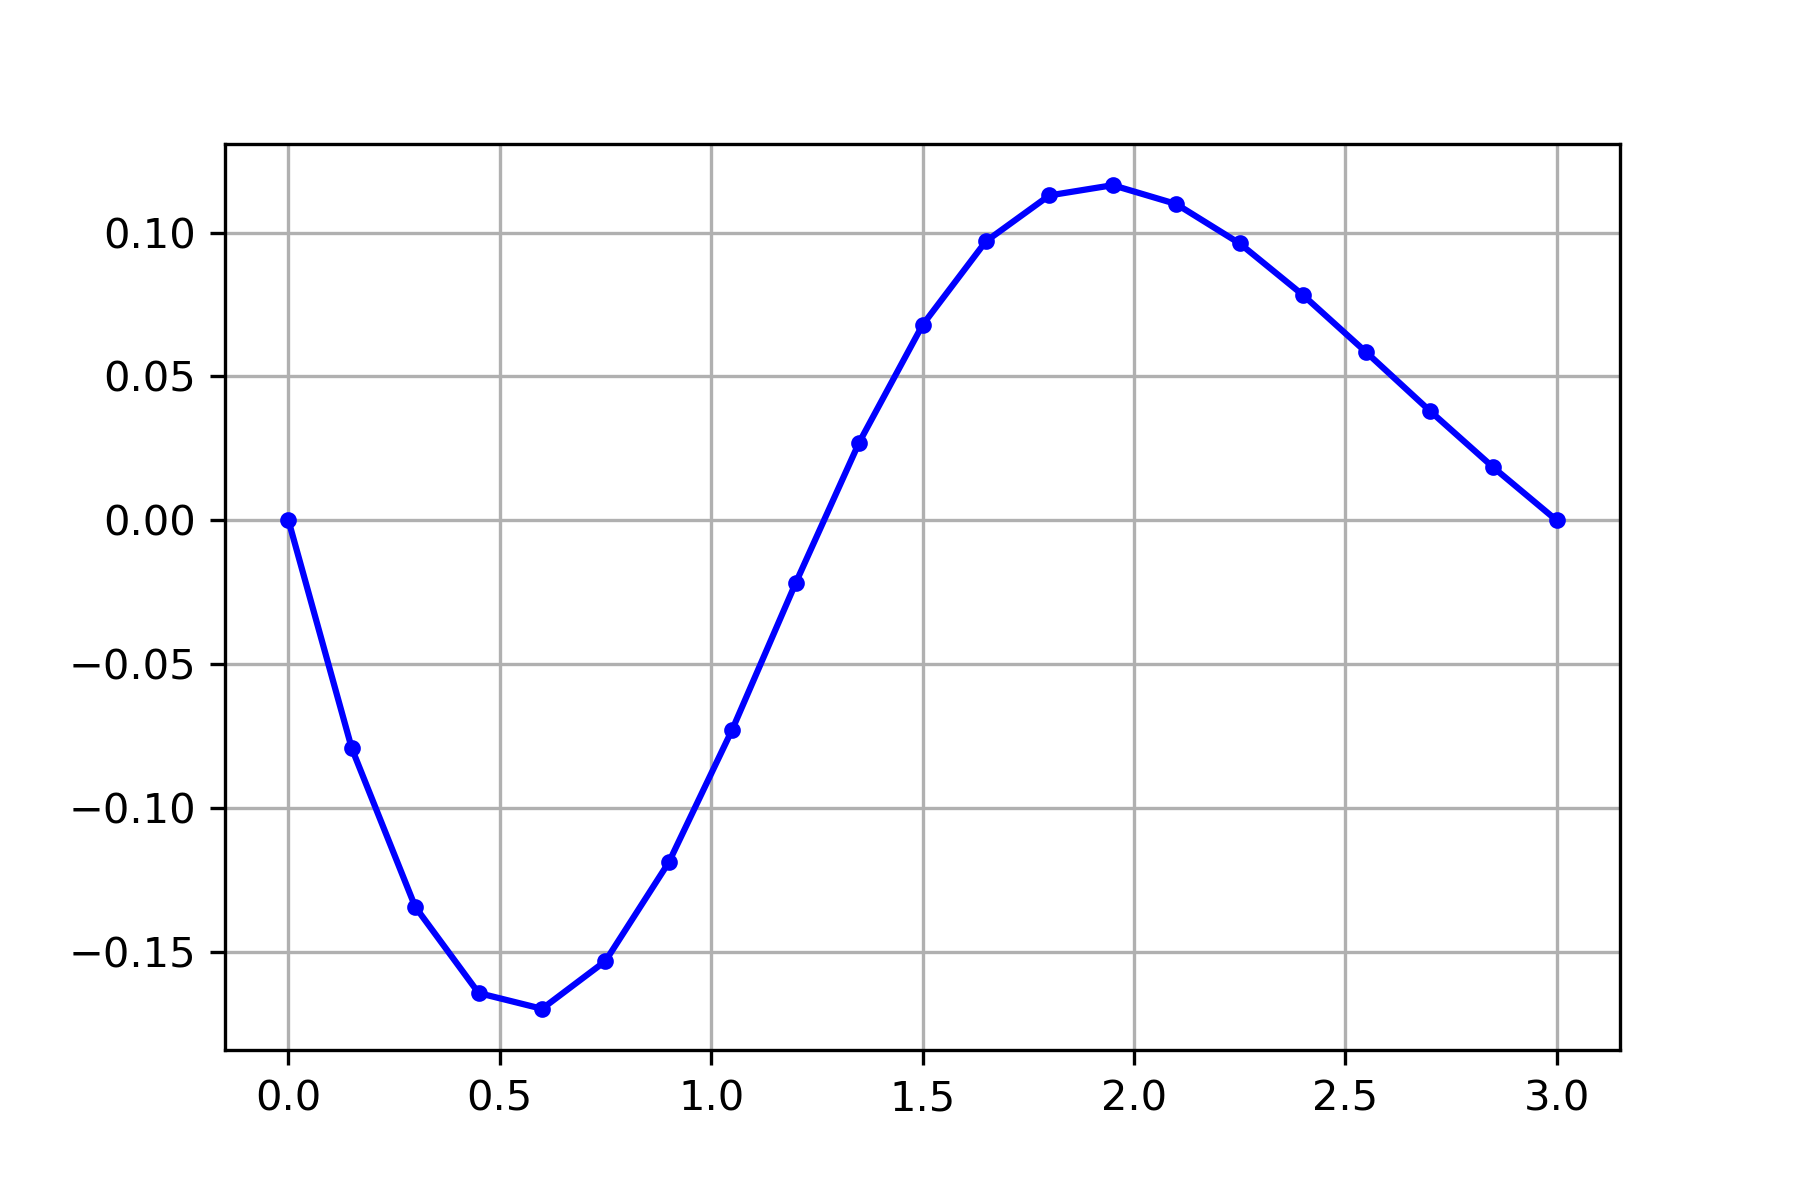
\includegraphics[width=4in]{01_08_img04.png}
\end{center}
\end{example}

\begin{example}
Consider a second order linear ordinary differential equation with boundary conditions of the form
$$
y'' = r(t) \ \ , \ \ y'(t_0) = \alpha \ , \ \ y(t_f) = \beta
$$
Note that the boundary condition at $t_0$ specifies the value of the derivative $y'(t_0) = \alpha$. Use the same notation as in the examples above and apply the central difference formula
$$
y_{k-1} -2y_k + y_{k+1} = h^2 r_k
$$
Therefore we have $N$ equations 
$$
\begin{array}{rrrrrrcrrrrrrcc}
y_0 & - & 2y_1 & + & y_2 & & & & & & & & & = & h^2 r_1 \\
& & y_1 & - & 2y_2 & + & y_3 & & & & & & & = & h^2 r_2 \\
& & & & & & \ddots & & & & & & & \vdots & \\
& & & & & & y_{N-2} & - & 2y_{N-1} & + & y_N & & & = & h^2 r_{N-1} \\
& & & & & & & & y_{N-1} & - & 2y_N & + & y_{N+1} & = & h^2 r_N
\end{array}
$$
We can use $y_{N+1} = \beta$ and move the term to the right side in the last equation but $y_0$ in the first equation is unknown. Use the forward difference formula to approximate $y_0$
$$
y'(t_0) \approx \frac{y(t_1) - y(t_0)}{h}
\ \ \Rightarrow \ \
y_0 = y_1 - h \alpha
$$
Therefore we can write the equations in matrix form $A \bs{y} = \bs{b}$ where
$$
A =
\left[ \begin{array}{rrcrr}
-1 & 1 & & & \\
1 & -2 & 1 & & \\
& & \ddots & & \\
& & 1 & -2 & 1 \\
& & & 1 & -2
\end{array} \right]
\hspace{10mm}
\bs{b} = 
\begin{bmatrix}
h^2 r_1 + h\alpha \\ h^2 r_2 \\ \vdots \\ h^2 r_{N-1} \\ h^2 r_N - \beta
\end{bmatrix}
$$
\end{example}